\documentclass{llncs}
\usepackage{amsmath,amssymb,algorithm,algorithmic}
\usepackage{hyperref,color}
% No page numbers.
\usepackage{subfig}
\usepackage{graphicx}

\newcommand{\tool}{\text{ANTsR}}
\newcommand{\R}{{\bf R}}
\newcommand{\X}{{\bf X}}
\newcommand{\Xh}{{\hat{{\bf X}}}}
\newcommand{\x}{{\bf x}}
\newcommand{\Y}{{\bf Y}}
% \newcommand{\U}{{\bf U}}
\newcommand{\V}{{\bf V}}
\newcommand{\E}{{\bf E}}
\newcommand{\y}{{\bf y}}
\newcommand{\Z}{{\bf Z}}
\newcommand{\z}{{\bf z}}
\newcommand{\bSigma}{\boldsymbol \Sigma}
\newcommand{\vect}[1]{\mathbf{#1}}
\newcommand{\field}[1]{\mathbf{#1}}
\newcommand{\image}[1]{#1}
\newcommand{\I}{\image{I}}
\newcommand{\J}{\image{J}}
\renewcommand{\u}{\vect{u}}
\renewcommand{\v}{\vect{v}}
\renewcommand{\c}{\vect{c}}
\newcommand{\h}{\vect{h}}
\newcommand{\w}{\vect{w}}
\newcommand{\myphi}{\phi}
\newcommand{\mypsi}{\psi}
\newcommand{\D}{D}
\renewcommand{\d}{\nabla}
\newcommand{\dd}{\text{d}}
\newcommand{\p}{\partial}
\renewcommand{\L}{\Delta} % laplacian
\newcommand{\myS}{S}
\newcommand{\myR}{R}
\newcommand{\myE}{E}
\newcommand{\ld}{\langle}
\newcommand{\rd}{\rangle}
\newcommand{\LL}{\mathcal{L}} % operator L
\newcommand{\tQ}{\mathcal{Q}}
\newcommand{\Id}{\text{Id}}
\newcommand{\tG}{{G}} % operator L
\newcommand{\Diff}{\text{Diff}}
\newcommand{\VV}{\mathcal{V}}
\newcommand{\opL}{\mathcal{L}}
\newcommand{\bs}{\boldsymbol}
\newcommand{\tk}{~ITK$^{\text{4}}$~}
\newcommand{\bsp}{$\substack{
   \rightsquigarrow \\
   b
  }$}
\newcommand{\mi}{$\substack{
   \approx \\
   \text{mi}
  }$}
\newcommand{\cc}{$\substack{
   \approx \\
   \text{cc}
  }$}
\usepackage{setspace,verbatim}
\begin{document}
\vspace{-0.1in}
\title{Standardized Registration Methods for the SATA Challenge Datasets}
\author{Brian B. Avants$^1$, Nicholas J. Tustison$^2$, Hongzhi
  Wang$^1$ \\and the
  $^5$\href{http://www.insightsoftwareconsortium.org/}{Insight Software Consortium}\\
$^1$Penn Image Computing and Science Lab \\ Dept. of Radiology \\University of
  Pennsylvania, Philadelphia, PA, 19104\\ 
  $^2$Dept. of Radiology and Medical Imaging, \\ University of Virginia,
  Charlottesville, VA 22903\\
 $^5$\href{http://www.insightsoftwareconsortium.org/}{http://www.insightsoftwareconsortium.org/}}
\maketitle              
\begin{abstract}
The 2012 Segmentation: Algorithms, Theory and Applications (SATA)
challenge suggests that even subtle variation in registration
performance may impact the outcome of multi-atlas segmentation
algorithms. The 2013 SATA challenge organizers therefore requested
standardized registration that enables entrants to use the same
mappings as input to competing algorithms.  We therefore collaborated
to provide, within a relatively brief window of time, over 22,000
registration results based on Advanced Normalization Tools
(\href{http://stnava.github.io/ANTs/}{ANTs link}).
The diencephalon component of the challenge presented familiar and
easily addressed data requiring only 1,600 mappings between different
3D human T1 neuroimages.  The 3D multiple modality MRI ``dog leg'' dataset ($>$ 7,000
mappings) presented the opportunity to improve performance by using
a multivariate similarity metric.  The 4D cardiac (or CAP) dataset
($\approx$ 13,000 mappings) includes highly variable image quality, anatomy
and field of view.  We detail the ANTs variants that address the most basic brain dataset, where we used
a template-based approach, to the more challenging CAP dataset which
employed a more customized registration solution based on prior
knowledge.  The scripts, source code and a small set of example data
accompany this paper and are available online.  
\footnote{This work is supported by National Library of Medicine sponsored ARRA stimulus
funding.}
\end{abstract}

\begin{comment}
Brian,
 
One of the results of our multi-atlas workshop / challenge was that registration often had a larger impact on method performance than the statistical combination method (no real surprise there: garbage in = garbage out). SyN was used by the top two groups using Arno Klein’s published parameters.
 
In our journal write-up of the workshop results, we are planning on re-running the fusion algorithms using a common registration. Would you be willing to provide the “definitive” SyN results? We have 15 source images (plus label maps) that we need to match pair-wise to 20 target images (without label maps). If you would prefer to specify the command line parameters, Andrew (cc’d) can run the data through on our system.
 
Thanks!
Bennett

Dr. Avants,

After last year's MICCAI whole-brain segmentation challenge, two things became abundantly clear: (1) in order to isolate the benefits of specific label fusion algorithms we need to have a standardized registration and (2) the ANTs registration package represents the premier image registration framework. 

As a result, for this year's challenge (as part of the SATA workshop ) we would like to provide standardized atlas-target registrations for each of the datasets that we are considering.

Would you be willing to contribute these standardized registrations for the challenge?

The workshop website can be found here:
https://masi.vuse.vanderbilt.edu/workshop2013/index.php/Main_Page

The information on each of the datasets can be found here:
https://masi.vuse.vanderbilt.edu/workshop2013/index.php/Segmentation_Challenge_Details

The complete data package can be downloaded here:
https://masi.vuse.vanderbilt.edu/workshop2013/index.php/SATA_Data_Registration_Form

 For this year's challenge we are considering 3 datasets:
(1) A diencephalon (mid-brain) dataset
(2) A canine leg dataset
(3) A cardiac atlas dataset

 ``From my perspective, I think that the mid-brain and canine leg
  datasets would not be terribly difficult to achieve consistent
  correspondence across the images. However, the cardiac atlas dataset
  might be significantly more challenging due to the way in which the
  images are acquired (i.e.,wildly varying orientations and
  fields-of-view).'' ---{\em SATA Organizers}

We would greatly appreciate your help for making this challenge as successful as possible. If you have any questions/comments/concerns please do not hesitate to bring them up.

Thanks again,
Andrew Asman

\end{comment}

\section{Introduction}
Several early papers in image registration / segmentation focus on 
clinical applications including microscopy, nuclear medicine, tracking longitudinal
change and angiography
\cite{Badran1991,Venot1986,Venot1984,Wrigley1982,Adair1981}.  Rapid progress in registration
theory and implementation followed these early developments with
focus, in general, on either similarity metrics \cite{Wells1996},
transformation models \cite{Miller2005} or the combination of these in a general
purpose method \cite{Rueckert1999}.  More recently, as the core technology of segmentation and
registration mature, the research focus has returned to specific clinical
applications such as radiation therapy \cite{Chan2013}, drug discovery \cite{Fox2009},
neurosurgery \cite{Omara2013} and image-based biomarkers of pain \cite{Loggia2013}.  
Quantitative image mapping is also relied upon heavily for automated analysis of large datasets
such as ADNI \cite{Weiner2012} that cannot be processed ``by hand.''

These new problem domains are revealing the limitations of traditional
methods.  Brain registration methods, for instance, often assume that
a single reference space / template is adequate to combine information
across a population and that there exists, roughly, a diffeomorphism
between any pair of individual brains.  Segmentation methods, on the
other hand, often assume that intensity and object smoothness or
texture encode the shape to be segmented or that a single model object
is sufficient to act as a prior.  These assumptions may not
hold when imaging other organs or in emerging MR modalities.  

Multi-atlas segmentation and registration (MASR) methods help overcome
the limitations associated with mapping to a single template or using
a single exemplar segmentation.  These methods encode the notion that
different topology or image contrast may exist between different
subjects and, further, that the user cannot know these subjects {\em a
priori}.  In this case, the problem is to develop algorithms that
automatically adjust for registration accuracy at both global and
local scales and determine segmentation labels that incorporate
confidence.  MASR therefore enables applications that do not depend upon
successful pair-wise registration between all subjects, a goal that is
currently beyond the reach of any general purpose registration tool.

The organizers of the SATA 2013 challenge collected datasets that
frame, with specific examples, the issues raised above.  The
organizers wrote on May 10, 2013 ``in order to isolate the benefits of
specific label fusion algorithms we need to have a standardized
registration.''  The ANTs development team agreed to collaborate on a set of standard registration results for the challenge.  We
felt that our participation was important due to the variety of the challenge
data, the fact that not all entrants are biomedical image registration
experts and the results of SATA 2012 which suggested that a common
transformation basis set would help isolate the differences between
the segmentation component in MASR.  In other words, using a common
set of ``voters'' allows a more direct comparison of the
segmentation/fusion methods that are currently at the heart of the
SATA challenge. We present,
below, the ANTs techniques that address the unique hurdles as well as
opportunities afforded by this diverse collection of images.

\section{Methods} 
Three MRI datasets constitute the driving biological problems for the
2013 challenge: T1-weighted whole head images of the diencephalon
(mid-brain), multi-modality T1 and T2 canine leg images and a 4D
cardiac atlas dataset.  The SATA organizers requested that we provide
transformed label sets and intensity images for all
training$\leftrightarrow$testing and training$\leftrightarrow$training
pairs.  The registration goal was to map the images with ``reasonable
and consistent'' peformance and an open-source system.  

We processed all data with Advanced Normalization Tools ( git commit
e3ba1c527fa63cc524bae7912b415d77adadc165 ) based on ITKv4.  The
processing was organized with a combination of bash or perl scripts
and run through standard Sun Grid Engine distributed computing.  The
core methods are available in ANTs programs \texttt{antsRegistration},
\texttt{ImageMath} (utilities), \texttt{N4BiasFieldCorrection} (bias
correction) and \texttt{Atropos} (segmentation).  These core tools are
described in archived publications
\cite{Tustison2010,Avants2011a,Avants2011}.  However, we employed
several new additions to ANTs registration that are as recent as 2013
and which are based upon our work for version 4 of the Insight
ToolKit. 

\subsection{The (Fire) ANTs System} ANTs fundamentals involve pairwise
registration of images defined in physical space.  ANTs registrations,
as of 2013 with the Fire beta, are defined by an initial transformation (possibly the
identity) of the ``fixed'' and/or ``moving'' images.  This is followed
by a series of registration stages typically with increasing degrees
of freedom.  Each stage begins with $k$ similarity metric definitions
(most often $k=1$) and is followed by parameters defining the
multi-resolution strategy.  Subsequent stages may be added in the same
style.  Finally, ANTs takes options controlling optimization details
and pre/post-processing.  Application-specific choices should be made
for the transformation, similarity metrics and multi-resolution
strategy.  A variety of options are exercised in SATA processing.

\subsection{Diencephalon/Brain Data (SATA-B)}
 \begin{quote}
 ``... the mid-brain and canine leg
  datasets should not be terribly difficult ...'' ---{\em SATA Organizers}
\end{quote}
\begin{figure}[t]
 \centering 
  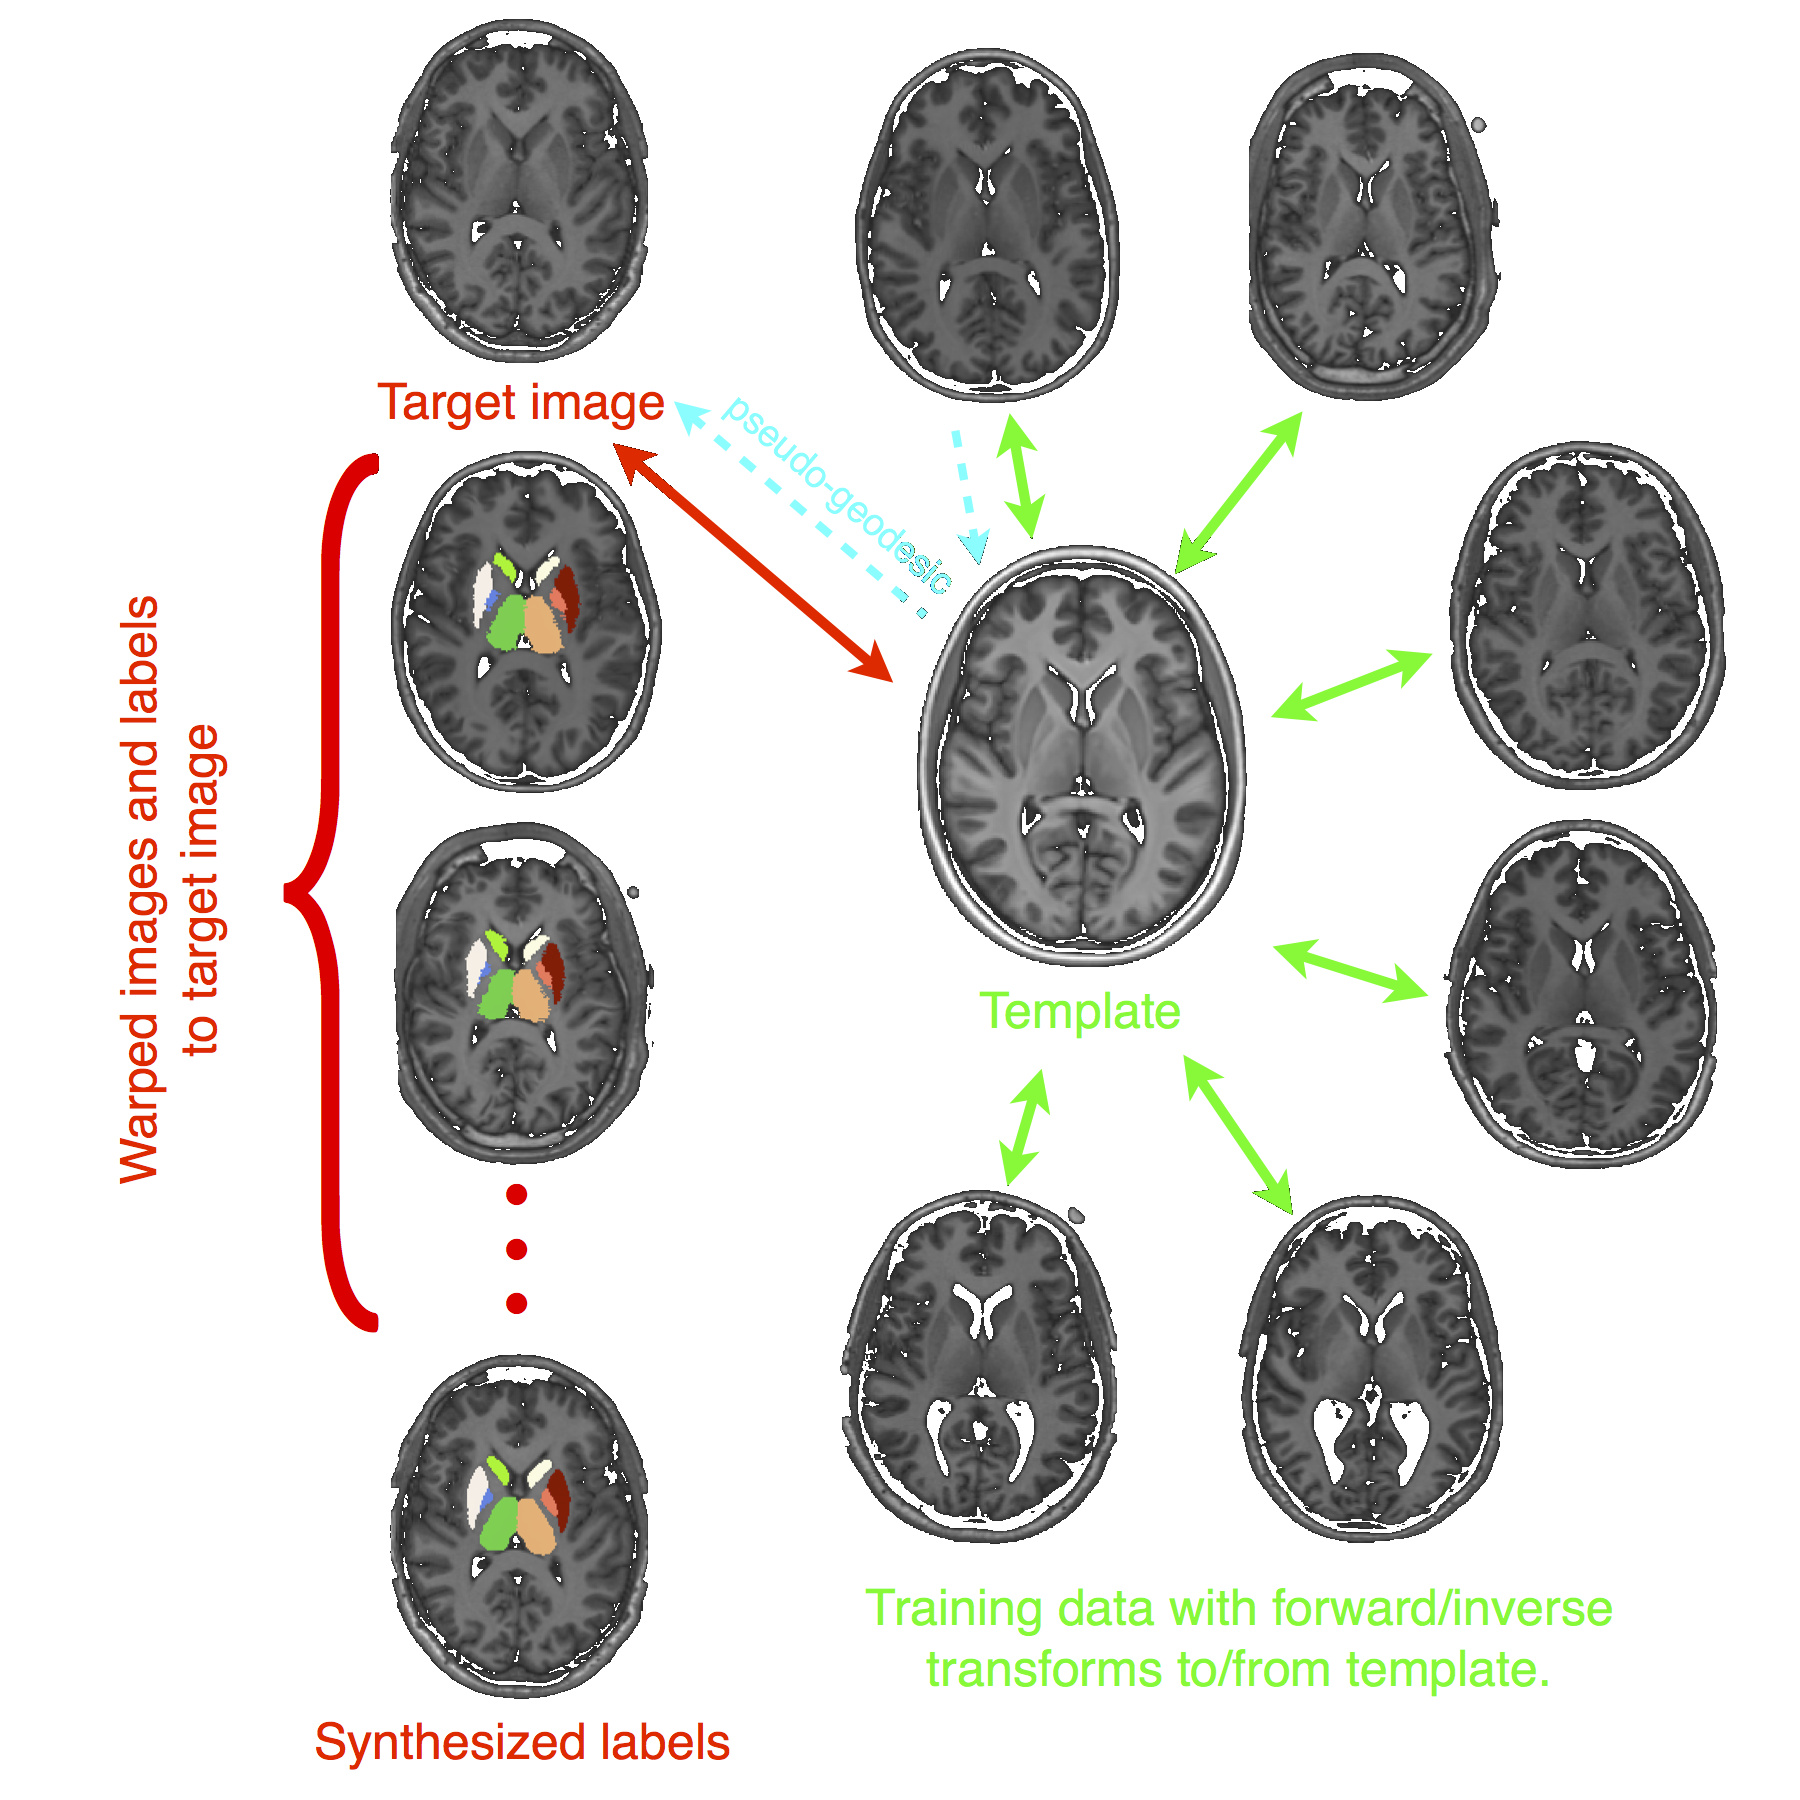
\includegraphics[width=3.5in]{../figs/SATA_diencephalon.png}
 \caption{SATA-B registrations map every image to every other image
   through the optimal template space (available online).  This
   requires only $n$ registrations rather than $n^2$.}
 \label{fig:Bmethods}
\end{figure}
We employed an efficient ``pseudo-geodesic'' processing strategy for this data to
avoid explicitly computing $\approx$1,600 image registration
instances, as shown in Figure~\ref{fig:Bmethods}.  As was shown in previous work (technical report), this
strategy improves upon single template labeling while approaching (not
equaling) the more computationally expensive all-pairs
registration required by standard MASR.

We first derive a custom whole-head template for this dataset and
extract the template cerebrum using MASR and LPBA40 labels \cite{Shattuck2008}.
We then extract the cerebrum from the individual SATA-B images based
on existing ANTs software (\texttt{extractBrainAllSubjects.pl}) for
template-based brain mapping.  We then re-registered the individual
cerebrum images to the template cerebrum
(\texttt{runSyNRegistrations.pl}).  The subject $n$ to template
mapping composes with the inverse of the subject $m$ to template
mapping to create the final mapping between subject $n$ and subject $m$.
The affine and deformable components of the SATA-B maps derive from
standard \texttt{antsRegistration} parameters.  
 
\subsection{Dog Leg Multi-Modality Data (SATA-L)}
\begin{figure}[t]
 \centering 
  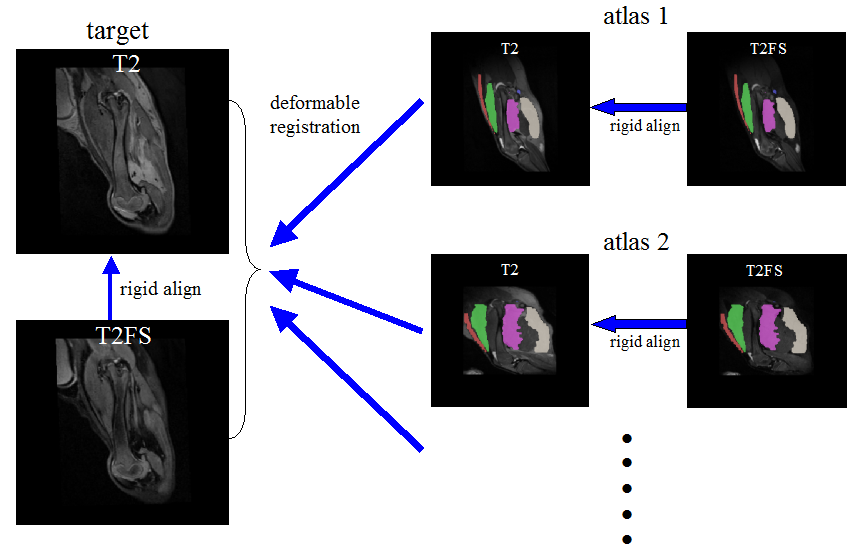
\includegraphics[width=3.5in]{../figs/canine-leg-registration.png}
 \caption{The SATA-L registration is similar to SATA-B.  However, the
image similarity is driven by the mutual information applied to both
modalities.  We chose to treat both modalities equally except for one
small detail---one of the modalities is rigidly registered,
intra-subject, to the other before proceeding with inter-subject
registration.}
 \label{fig:Lmethods}
\end{figure}
The input modalities are
bias corrected by N4 \cite{Tustison2010} before further processing (\texttt{normalization.sh}).  ANTs
registration employs both modalities provided for SATA-L.  We did not
know the relative contribution of each modality to accuracy so set
equal weights.  The affine and deformable components of the SATA-L
maps derive from a multivariate extension to standard
\texttt{antsRegistration} parameters.  That is, we use the standard
multi-resolution affine approach combined with SyN but drive both
transformation stages by the sum of mutual information across both
modalities.  More specifically, for affine registration, we optimize:
\begin{eqnarray}
w_1 MI(  I_1 , J_1( \phi(x) ) ) +
w_2 MI(  I_2(\psi_I(x)) , J_2( \psi_J(\phi(x)) ) ) \notag \\ 
\text{Subject to:}~\phi \in Diff_\text{Affine},
\end{eqnarray}
where $w_1=w_2=0.5$ and $\psi_J$ rigidly maps $J_2$ to $J_1$
(similarly $\psi_I$).  The script \texttt{align.sh} shows how to
compute $\psi$.  We use the same multivariate metric for SyN deformable mapping (\texttt{registerPairsMod.sh}).  Note that
\texttt{antsRegistration} allows initial mappings to be provided thus
reducing accumulation of interpolation error.  Five percent regular
subsampling of the joint intensities estimates the mutual information
metric and metric derivative.
% FIXME --- are $I_1$ and $I_2$ in alignment?

\subsection{CAP Cardiac Data (SATA-C)}
The CAP dataset is more challenging than the other two and includes a volumetric time series of the beating heart:
 \begin{quote}
  `` ... I wouldnt be surprised if getting `reasonable' \& `consistent' registrations for this data is difficult or impossible.'' ---{\em SATA Organizers}
\end{quote}
\noindent The dataset indeed proves to be challenging to process with
a general purpose toolkit like ANTs.  Our procedure is illustrated
with example data in 
\url{https://github.com/stnava/LabelMyHeart} \footnote{May not be the
  exact scripts used due to a few last minute changes stored on the
  distributed computing system.}

\begin{figure}[t]
 \centering 
  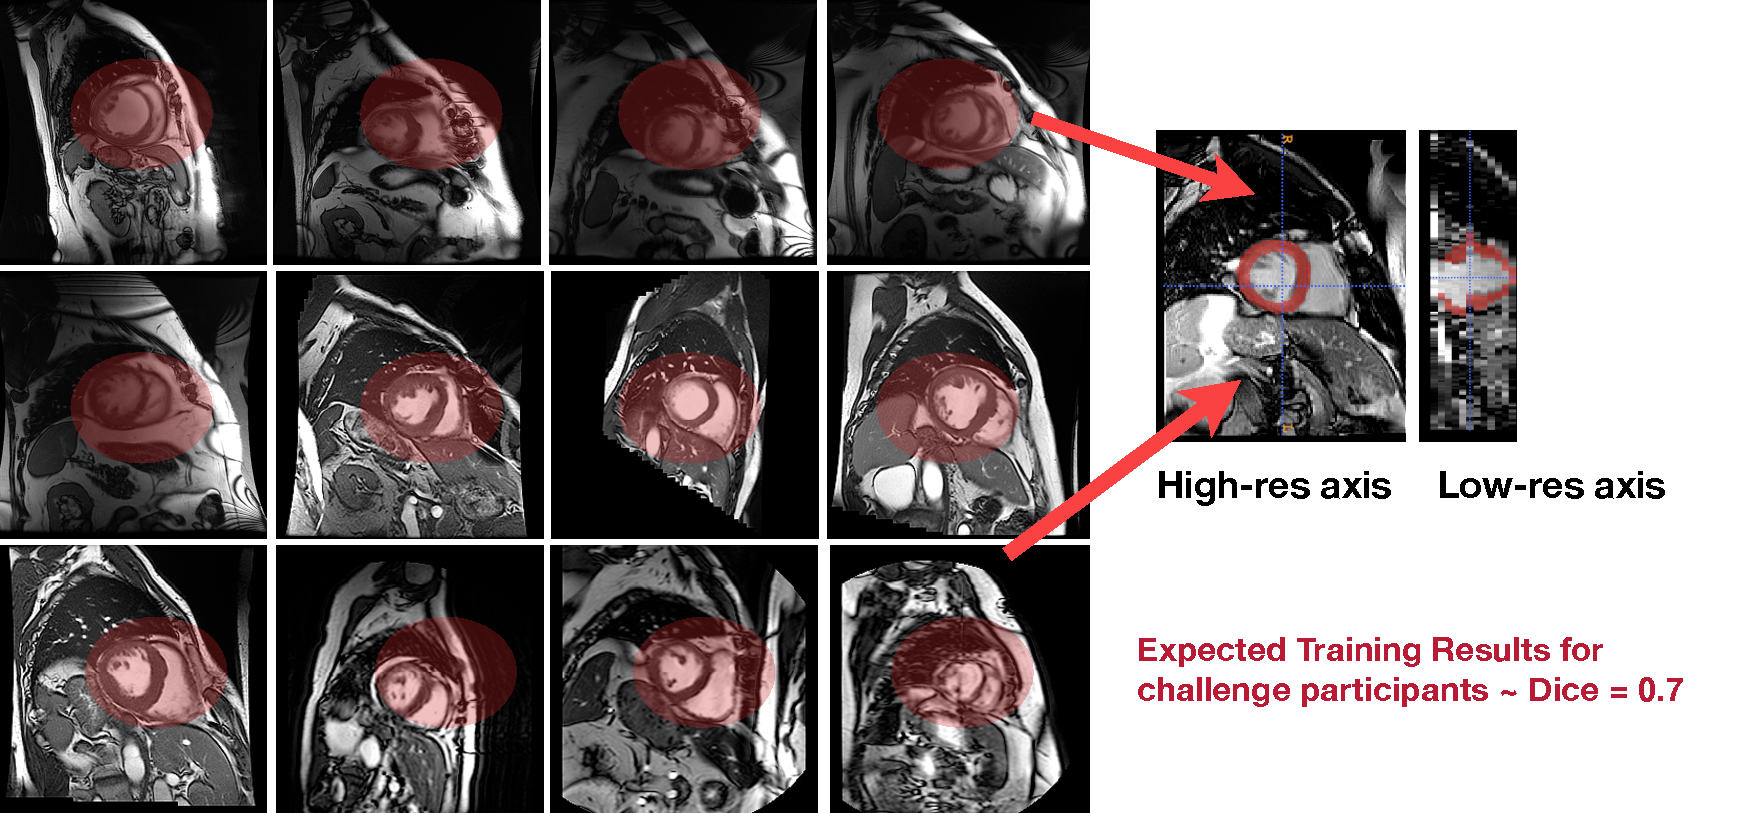
\includegraphics[width=5in]{../figs/CAP_methods.pdf}
 \caption{CAP methods}
 \label{fig:CAPmethods}
\end{figure}

\begin{figure}[t]
 \centering 
  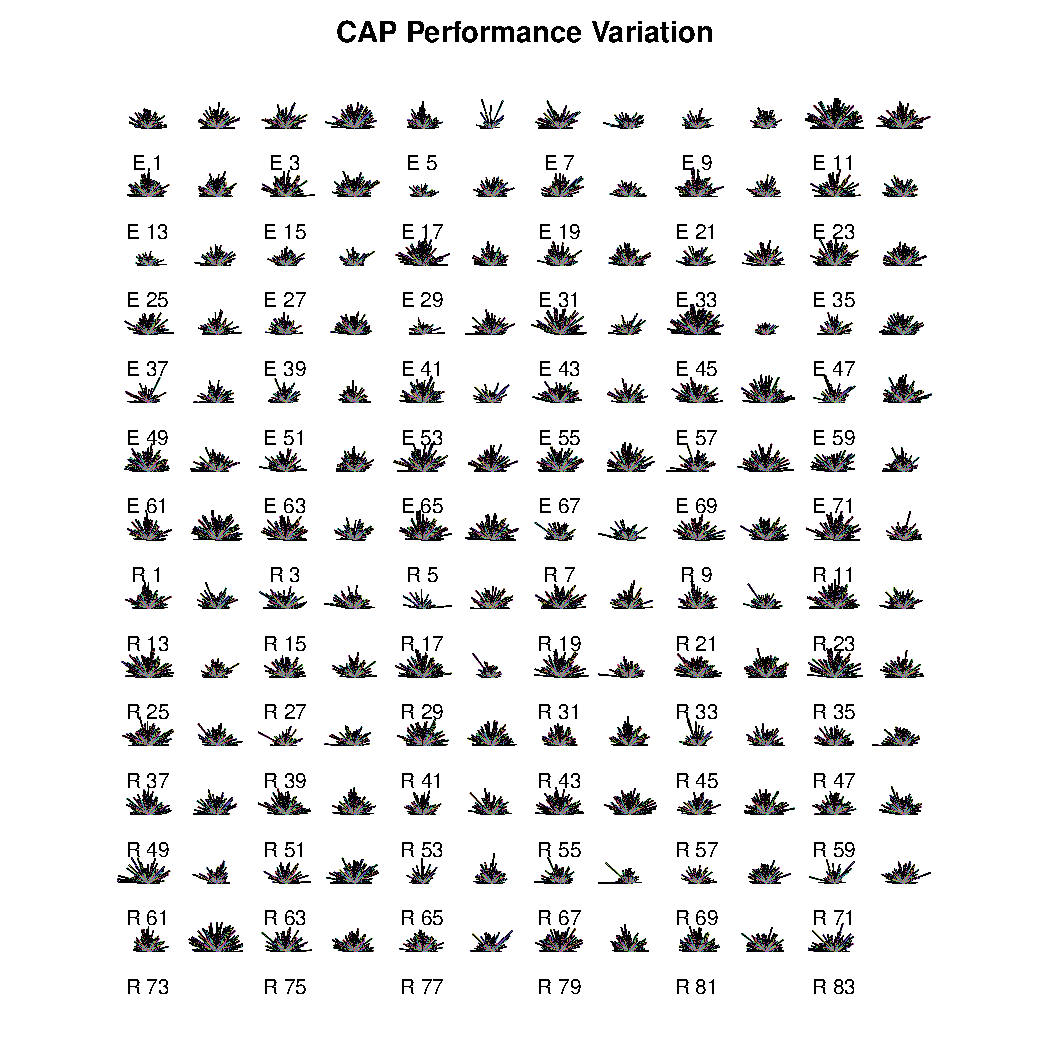
\includegraphics[width=5in]{../figs/spider_CAP.pdf}
 \caption{We use urchin plots to visualize pairwise registration
   performance for CAP data.  We quantified variability in
   all 12,865 data points by measuring
   the global correlation of the deformed image and the target image,
   i.e. both training (labeled R$\star$) and testing (labeled E$\star$). ``Spiky''
   distributions of the correlation function indicate that
 a few pairings performed much better/worse than the majority, at
 least at a global level.  This
 was verified by testing the gaussianity of the resulting correlation
 distribution.  As an example, the sixth subject from top left (E6) has a
 highly non-gaussian distribution of similarity metric performance and
results in a significant p-value for the non-gaussianity test ($p <$
1.e-7 ).  Overall, 13.5\% of subjects exhibited non-gaussian
distributions for this function, after multiple comparisons correction by false discovery rate.}
 \label{fig:CAPvar}
\end{figure}

\section{Results}

\subsection{Diencephalon/Brain Data}

\subsection{Dog Leg Multi-Modality Data}

\subsection{CAP Cardiac Data}
We estimated a failure rate of X\% on this data  .... look at
histogram of correlation 

\section{Discussion} The processing decisions that we made in the
standard registration suggest several possible outcomes.  For
instance, our pseudo-geodesic approach focusing on the whole brain
should be suboptimal for the the diencephalon data. Entrants that
choose to perform pairwise registration between all subjects should
find better performance than the standard approach.

The cardiac dataset reveals some of the limitations involved with
naive pair-wise registration and highlights the benefit of
problem-specific strategies and multi-atlas methods.  We believe that,
of the 3 datasets, the biggest future performance gains may be
possible in this type of data.  While the organizers requested that
the output labels be consistent with the original 4D manual labels,
the intra-rater variability in labeling the time series in unknown; at
first glance, it would seem difficult to consistently label the
myocardium in 3D over several dozen or more time frames.  Therefore,
the upper limits on accuracy remain unclear.

\bibliographystyle{splncs}
\bibliography{knobsock}
\end{document}



